\documentclass[conference,a4paper]{IEEEtran}
\IEEEoverridecommandlockouts
\usepackage{cite}
\usepackage{amsmath,amssymb,amsfonts}
\usepackage{algorithmic}
\usepackage{algorithm}
\usepackage{graphicx}
\usepackage{textcomp}
\usepackage{xcolor}
\usepackage{booktabs}
\usepackage{url}
\def\BibTeX{{\rm B\kern-.05em{\sc i\kern-.025em b}\kern-.08em
    T\kern-.1667em\lower.7ex\hbox{E}\kern-.125emX}}

\begin{document}

\title{Hybrid CLAHE--Retinex Enhancement for\\ Nighttime Surveillance Images}

\author{\IEEEauthorblockN{Bekir Erakb{\i}y{\i}k}
\IEEEauthorblockA{\textit{Department of Computer Engineering} \\
\textit{Student ID: 2211051073} \\
Digital Image Processing -- Term Project \\
bekir.erakbiyik@agu.edu.tr}}

\maketitle

\begin{abstract}
Images captured by nighttime surveillance cameras suffer from low contrast,
poor visibility, and signal-dependent sensor noise that degrade downstream
vision tasks such as object detection and license-plate recognition. Global
enhancement methods tend to over-amplify noise in dark regions, whereas
Retinex-based methods recover detail but introduce halo artifacts and color
shifts. This paper proposes a hybrid pipeline that combines Contrast Limited
Adaptive Histogram Equalization (CLAHE) and Single Scale Retinex (SSR) in the
Value (V) channel of the HSV color space, leaving hue and saturation untouched
to preserve natural color. Unlike prior CLAHE--Retinex fusions that blend the
two branches with fixed, hand-picked global weights, we introduce a
\emph{content-adaptive} fusion in which the per-pixel weight is derived from a
local illumination estimate: the noise-bounded CLAHE branch dominates dark
regions while the reflectance-recovering SSR branch is favored where it is safe.
The method is compared against Global Histogram Equalization (GHE), fixed Gamma
correction, the CLAHE-only and SSR-only branches, and a fixed-weight fusion
baseline. On a synthetic low-light benchmark built from the Kodak image suite
(five reference images, three noise realizations each), the adaptive method
attains the best fidelity, reaching $19.03$\,dB PSNR versus $18.39$\,dB for the
fixed-weight fusion and $17.09$\,dB for the next-best classical baseline (GHE),
and it ranks first on every individual image. A hyperparameter study over the
CLAHE clip limit, SSR Gaussian scale, and the single adaptive exponent
characterizes the contrast--fidelity trade-off. Source code is publicly
available.
\end{abstract}

\begin{IEEEkeywords}
low-light image enhancement, CLAHE, Retinex, image fusion, HSV color space,
nighttime surveillance, PSNR, SSIM, BRISQUE
\end{IEEEkeywords}

\section{Introduction}
Low-light image enhancement is a long-standing problem in computer vision and
is particularly critical for nighttime surveillance, where images captured
under weak illumination exhibit poor visibility, compressed dynamic range, and
strong sensor noise. These degradations reduce the reliability of automated
tasks such as object detection, tracking, and license-plate recognition. The
core difficulty is a fundamental trade-off: brightening dark regions
simultaneously amplifies the noise that dominates those regions, while overly
aggressive enhancement near bright light sources (street lamps, headlights)
produces halo artifacts and unnatural colors.

Classical contrast-stretching approaches such as Global Histogram Equalization
(GHE) redistribute intensities over the whole image; they raise global contrast
but ignore local structure and amplify background noise in dark areas. Fixed
Gamma correction is a simple nonlinear brightness mapping, but a single global
exponent cannot adapt to scenes that contain both very dark and bright regions
at once. The relevant prior art on adaptive and Retinex-based enhancement is
reviewed in Section~\ref{sec:related}.

\textbf{Research gap.} Contrast-oriented methods raise background noise, whereas
Retinex-oriented methods add halos and color distortion, motivating hybrid
CLAHE--Retinex pipelines. However, existing hybrids typically combine the two
branches with a single \emph{fixed, global} weight (or a manually tuned constant
blend) applied uniformly to every pixel. This is sub-optimal because the
reliability of each branch is \emph{spatially varying}: in dark regions the
SSR log-ratio strongly amplifies sensor noise and the bounded-contrast CLAHE
output is preferable, whereas in well-lit regions CLAHE adds little and SSR can
safely recover reflectance detail. A globally fixed weight cannot exploit this
spatial structure, and the specific weight values are usually left unjustified.
The gap we address is therefore the absence of a \emph{principled, content-adaptive}
fusion rule that varies the CLAHE/SSR contribution per pixel according to local
image evidence, while remaining lightweight and training-free and preserving
natural color.

\textbf{Contribution.} This work makes the following contributions:
\begin{itemize}
\item A \emph{content-adaptive} CLAHE--Retinex fusion that, instead of a fixed
global weight, sets the per-pixel CLAHE/SSR weight from a local illumination
estimate via a single interpretable exponent, so that the noise-bounded branch
dominates dark regions and the detail-recovering branch is favored where safe.
The fusion operates only on the V channel so that hue and saturation -- and
hence color -- are preserved.
\item A controlled comparison against two classical baselines (GHE, Gamma), an
ablation against the individual CLAHE-only and SSR-only branches, \emph{and a
fixed-weight fusion baseline}, isolating the benefit of adaptivity itself, all
evaluated with full-reference (PSNR, SSIM) and no-reference (BRISQUE) metrics
plus runtime.
\item A hyperparameter study over the CLAHE clip limit, the SSR Gaussian scale,
and the adaptive fusion exponent, quantifying how each factor moves the
contrast--fidelity trade-off, together with publicly released code.
\end{itemize}

\section{Related Work}
\label{sec:related}
\textbf{Histogram-based enhancement.} Histogram equalization remaps intensities
so the output histogram is approximately uniform. Its global form (GHE) is fast
but spatially blind. Adaptive Histogram Equalization
(AHE)~\cite{pizer1987ahe} equalizes small tiles to improve local contrast, but
in flat regions the steep local mapping over-enhances noise. Contrast Limited
AHE (CLAHE)~\cite{zuiderveld1994clahe} clips each local histogram at a fixed
limit before equalization and redistributes the excess, bounding the slope of
the mapping and therefore the noise gain; bilinear interpolation across tiles
removes block artifacts. CLAHE is widely used in medical and surveillance
imaging because of this controllable behavior, but on its own it neither
brightens severely under-exposed scenes nor compresses dynamic range.

\textbf{Retinex-based enhancement.} Retinex theory~\cite{jobson1997retinex}
models a captured image as the product of illumination and reflectance and
estimates the perceptually relevant reflectance by removing a low-pass estimate
of the illumination. Single Scale Retinex (SSR) uses one Gaussian surround;
multi-scale variants combine several scales for better rendition. Retinex
methods compress dynamic range and reveal shadow detail effectively, but the
center--surround subtraction tends to create halos around strong edges and can
shift colors when the gray-world assumption fails.

\textbf{Learning-based enhancement.} Recent deep methods such as
Zero-DCE~\cite{guo2020zerodce} treat enhancement as image-specific curve
estimation and achieve strong perceptual results without paired data. However,
they require model training, larger compute, and careful loss design, which can
be impractical for lightweight, on-device nighttime surveillance. Our work
instead targets a training-free pipeline whose few parameters are
interpretable, while borrowing the central insight that contrast restoration and
illumination/reflectance modeling are complementary and best combined rather
than used in isolation.

\section{Materials and Methods}

\subsection{Dataset and Low-Light Protocol}
Full-reference metrics such as PSNR and SSIM require a clean ground-truth
reference. Because raw low-light captures do not provide such references, we
adopt the widely used \emph{synthetic degradation} protocol: well-exposed
natural images are darkened and corrupted with sensor noise, enhanced, and then
compared against the original clean image. We use five reference images from the
Kodak Lossless True Color Image Suite, a standard natural-scene benchmark, and
resize them so that the longest side is at most $512$\,px.

The degradation operates on normalized intensities $I\in[0,1]$ and combines
under-exposure with signal-dependent noise:
\begin{align}
I_{\text{dark}} &= s \cdot I^{\gamma_d}, \\
I_{\text{low}}  &= \mathcal{P}\!\left(I_{\text{dark}}\cdot Q\right)/Q
                   + \mathcal{N}(0,\sigma_r^2),
\end{align}
where $\gamma_d>1$ compresses bright values toward zero, $s\in[0,1]$ lowers the
mean brightness, $\mathcal{P}(\cdot)$ is a Poisson process modeling photon
shot noise with photon scale $Q$, and $\mathcal{N}(0,\sigma_r^2)$ is additive
Gaussian read noise. We use $\gamma_d=2.2$, $s=0.6$, $Q=400$, and
$\sigma_r=0.01$. Shot noise scales with intensity, so dark regions have the
lowest signal-to-noise ratio, mimicking real CMOS sensors. Three noise
realizations are generated per image (seeds $0$--$2$), giving $15$ degraded
samples in total.

\subsection{Why the HSV Value Channel}
A central design choice is to enhance only the luminance and to do so in HSV
rather than in RGB. Applying CLAHE or Retinex independently to the R, G, and B
channels alters the ratios between them, which shifts hue and produces the
desaturated or color-cast results commonly seen with naive per-channel
enhancement. By converting to HSV, isolating the Value channel, enhancing it,
and recombining it with the \emph{unchanged} Hue and Saturation, the proposed
pipeline modifies brightness and contrast while leaving the chromatic content
intact. This is particularly important for surveillance, where color cues
(vehicle color, clothing) carry forensic value and must not be distorted by the
enhancement. The same argument motivates fusing the two branches in the V
domain only: both $V_{\text{CLAHE}}$ and $V_{\text{SSR}}$ are single-channel
luminance maps, so their weighted average is well defined and cannot introduce
new chromatic artifacts.

\subsection{Baseline Methods}
\textbf{Global Histogram Equalization (GHE).} The cumulative distribution of the
V channel is used as an intensity remapping so that the output histogram is
approximately uniform. It increases global contrast but ignores spatial context
and amplifies noise in dark regions.

\textbf{Gamma correction.} A fixed nonlinear mapping
$V_{\text{out}} = 255\,(V/255)^{\gamma}$ is applied to the V channel. We use
$\gamma=0.5$ to brighten. A single global $\gamma$ cannot simultaneously serve
dark and bright regions.

\subsection{Proposed Hybrid CLAHE--Retinex Method}
The proposed pipeline (Fig.~\ref{fig:pipeline}) processes only the luminance to
avoid color distortion. Given a BGR image, we convert to HSV and extract the
V channel. CLAHE and SSR are then applied \emph{independently} to the same
single V channel (neither branch sees the other's output); the two resulting
luminance maps are combined afterwards by the fusion rule defined below.

\emph{CLAHE branch.} CLAHE divides V into $8\times8$ tiles and equalizes each
local histogram after clipping it at a clip limit $\beta$, redistributing the
clipped mass uniformly. Bilinear interpolation across tiles removes block
boundaries. This yields $V_{\text{CLAHE}}$ with enhanced local contrast and
bounded noise gain.

\emph{SSR branch.} Single Scale Retinex estimates the log-reflectance by
subtracting a Gaussian-blurred (surround) version of the log-luminance:
\begin{equation}
R(x,y) = \log\!\big(V(x,y)+1\big) - \log\!\big(G_\sigma * V (x,y)+1\big),
\end{equation}
where $G_\sigma$ is a Gaussian of standard deviation $\sigma$ and $*$ denotes
convolution. The result is robustly min--max normalized (using the $1$st and
$99$th percentiles to resist outliers) back to $[0,255]$, giving
$V_{\text{SSR}}$, which recovers shadow detail and compresses dynamic range.

\emph{Fusion.} The two branches are applied independently to the same V channel
and then combined by a \emph{per-pixel} convex sum. Rather than choosing a
single global weight, we let the weight depend on the local image content. We
first form a smoothed illumination estimate by Gaussian-blurring the luminance,
\begin{equation}
L(x,y) = \frac{(G_\sigma * V)(x,y)}{255} \in [0,1],
\end{equation}
which is large in well-lit regions and small in dark regions. The per-pixel
SSR and CLAHE weights are then
\begin{equation}
w_S(x,y) = L(x,y)^{k}, \qquad w_C(x,y) = 1 - w_S(x,y),
\end{equation}
with a single exponent $k>0$, and the fused luminance is the convex combination
\begin{equation}
V_{\text{fused}}(x,y) = w_C(x,y)\,V_{\text{CLAHE}}(x,y)
                       + w_S(x,y)\,V_{\text{SSR}}(x,y).
\end{equation}
The design is principled: because $L\in[0,1]$, raising it to the power $k$ keeps
$w_S$ small in dark regions (so the noise-bounded CLAHE output dominates exactly
where SSR would amplify noise most) and lets $w_S$ grow toward bright,
well-exposed regions (where SSR can safely restore reflectance detail). The
exponent $k$ controls how quickly SSR is suppressed as a region darkens: larger
$k$ confines SSR to brighter areas. This replaces the three hand-picked global
weight pairs of a fixed blend with one interpretable parameter that is tuned by
the same metric-driven search used for the other hyperparameters
(Section~\ref{sec:results}). A fixed-weight fusion $V_{\text{fused}} =
w_C V_{\text{CLAHE}} + w_S V_{\text{SSR}}$ with constant $w_C,w_S$ is retained as
an explicit baseline to isolate the contribution of adaptivity.

Finally, $V_{\text{fused}}$ replaces the original V channel, and the image is
converted back to BGR using the untouched H and S channels, preserving the
original color appearance. The default operating point is $\beta=4.0$,
$\sigma=30$, $k=0.35$. The full procedure is summarized in
Algorithm~\ref{alg:hybrid}.

\begin{algorithm}[t]
\caption{Content-Adaptive CLAHE--Retinex (V-channel fusion)}
\label{alg:hybrid}
\begin{algorithmic}[1]
\REQUIRE BGR image $I$; clip limit $\beta$; scale $\sigma$; exponent $k$
\STATE $(H,S,V) \leftarrow \textsc{BGRtoHSV}(I)$
\STATE $V_{\text{CLAHE}} \leftarrow \textsc{CLAHE}(V,\ \beta,\ 8\times8)$
\STATE $L_{\log} \leftarrow \log(V+1)$;\quad $A \leftarrow \log(G_\sigma * V + 1)$
\STATE $R \leftarrow L_{\log} - A$ \COMMENT{single-scale Retinex on V}
\STATE $V_{\text{SSR}} \leftarrow \textsc{PercentileNorm}(R,\ 1\%,\ 99\%)$
\STATE $L \leftarrow (G_\sigma * V)/255$ \COMMENT{per-pixel illumination in $[0,1]$}
\STATE $w_S \leftarrow L^{k}$;\quad $w_C \leftarrow 1 - w_S$
\STATE $V_{\text{fused}} \leftarrow w_C \odot V_{\text{CLAHE}} + w_S \odot V_{\text{SSR}}$
\STATE \textbf{return} $\textsc{HSVtoBGR}(H,\ S,\ \textsc{clip}(V_{\text{fused}}))$
\end{algorithmic}
\end{algorithm}

\textbf{Computational complexity.} For an image with $N$ pixels, CLAHE is
$O(N)$ (per-tile histograms plus bilinear interpolation), and the dominant cost
is the Gaussian surround of SSR. Using OpenCV's separable Gaussian, the SSR
branch is $O(N)$ as well but with a larger constant due to two $1$D passes and
the logarithm/exponential operations. The adaptive fusion adds one extra
Gaussian blur for the illumination map plus an $O(N)$ per-pixel weighting, so
the total is still linear in image size. The method needs no training or GPU,
which suits embedded surveillance hardware; the measured per-image runtime
(Section~\ref{sec:results}) is dominated by the Gaussian convolutions.

\begin{figure}[t]
\centering
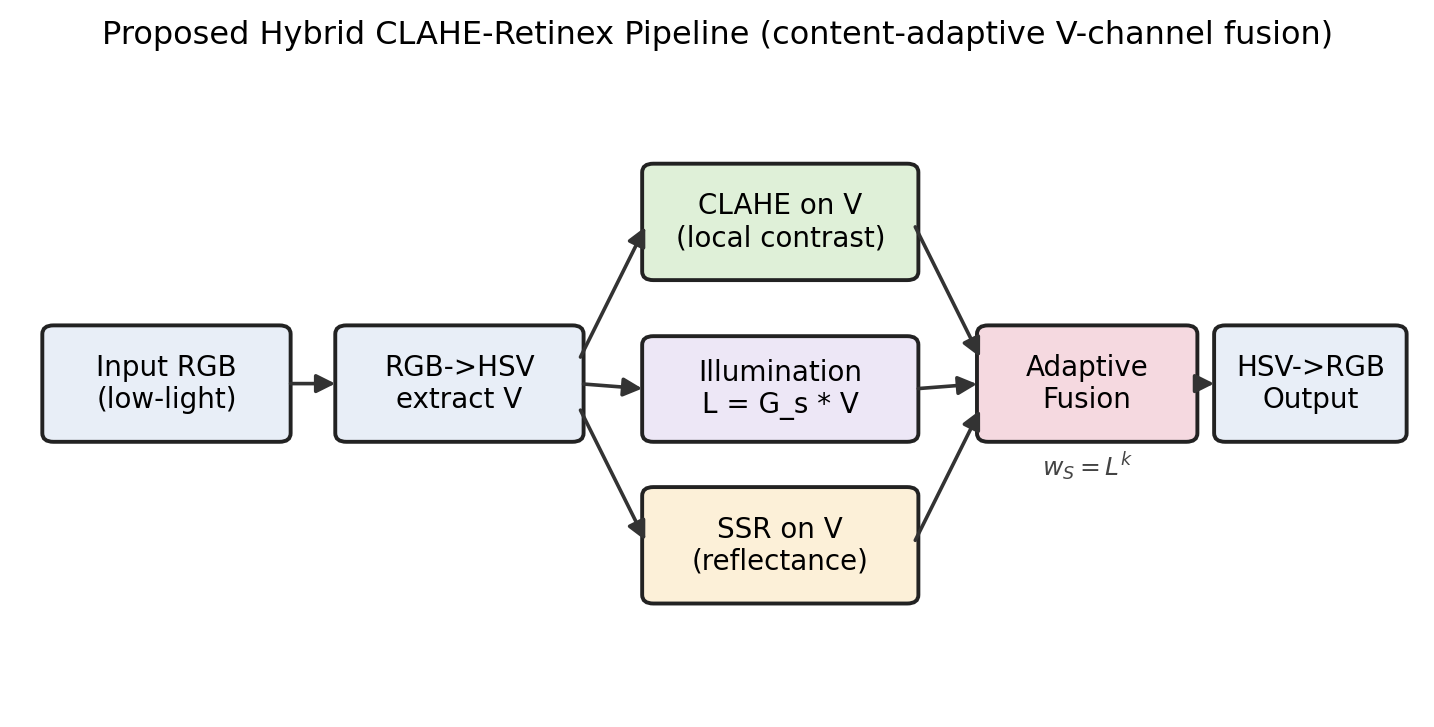
\includegraphics[width=\columnwidth]{fig_pipeline.png}
\caption{Proposed content-adaptive CLAHE--Retinex pipeline. Only the HSV Value
channel is processed; CLAHE supplies bounded local contrast and SSR supplies
reflectance/detail. A per-pixel illumination estimate $L$ drives the fusion
weight $w_S=L^{k}$, so SSR is favored in bright regions and CLAHE in dark ones,
before the image is converted back to RGB.}
\label{fig:pipeline}
\end{figure}

\subsection{Evaluation Metrics}
We report two full-reference metrics -- Peak Signal-to-Noise Ratio
(PSNR, higher is better, quantifying noise/fidelity) and the Structural
Similarity Index (SSIM~\cite{wang2004ssim}, higher is better) -- and one
no-reference metric, BRISQUE~\cite{mittal2012brisque} (lower is better, a
natural-scene-statistics measure of perceptual quality). We additionally report
grayscale entropy (information content) and per-image runtime. NIQE
\cite{mittal2013niqe} is a related no-reference alternative. The implementation
uses Python with OpenCV, NumPy, and scikit-image, and is runnable in Google
Colab.

\section{Experimental Results}
\label{sec:results}

\subsection{Parameter Settings}
Unless otherwise stated, all methods use the default operating point above.
GHE has no parameters; Gamma uses $\gamma=0.5$; the CLAHE-only and SSR-only
ablation branches use the same $\beta$ and $\sigma$ as the proposed method. The
fixed-fusion baseline uses constant weights $w_C=0.6$, $w_S=0.4$, and the
proposed adaptive method uses exponent $k=0.35$. Results are averaged over the
$5$ Kodak images $\times\,3$ noise realizations, and we report mean and standard
deviation.

\subsection{Quantitative Comparison}
Table~\ref{tab:summary} summarizes the results. The degraded input (no
enhancement) sits at $10.14$\,dB PSNR with low entropy, confirming a severe
low-light condition. The proposed adaptive method achieves the highest PSNR
($19.03$\,dB), exceeding the fixed-weight fusion ($18.39$\,dB) by $0.64$\,dB,
the strongest classical baseline GHE ($17.09$\,dB) by $1.94$\,dB, and the
SSR-only branch by $3.33$\,dB. The gain over the fixed-fusion baseline is the
key result: it isolates the benefit of \emph{adaptivity} alone, since the two
methods share identical branches and differ only in how the weights are chosen.
Gamma attains the best SSIM ($0.513$) because its smooth global mapping
introduces no new structure, but it leaves the image dark and noisy in shadow
regions, as the qualitative results show; the adaptive method matches the
fixed-fusion SSIM ($0.494$) while improving fidelity. On BRISQUE the adaptive
method ($51.7$) stays close to the fixed fusion and well below the artifact-prone
SSR-only branch ($55.8$), confirming that the per-pixel weighting does not
reintroduce the perceptual artifacts of pure Retinex. The method runs in about
$78$\,ms per image, roughly double the single-branch SSR cost because of the
extra illumination-map convolution; the CLAHE branch alone is a few
milliseconds.

\begin{table}[t]
\centering
\caption{Average results over 5 Kodak images $\times$ 3 noise realizations.
Arrows indicate the better direction. Best value per column in \textbf{bold}.}
\label{tab:summary}
\setlength{\tabcolsep}{4pt}
\begin{tabular}{lccccc}
\toprule
Method & PSNR$\uparrow$ & SSIM$\uparrow$ & BRISQUE$\downarrow$ &
Entropy$\uparrow$ & Time (ms) \\
\midrule
Low-light (input) & 10.14 & 0.290 & \textbf{22.8} & 6.04 & --- \\
GHE               & 17.09 & 0.454 & 49.9 & \textbf{7.79} & \textbf{1.8} \\
Gamma             & 15.50 & \textbf{0.513} & 45.3 & 6.93 & 1.8 \\
CLAHE-only        & 15.55 & 0.483 & 47.5 & 7.36 & 2.8 \\
SSR-only          & 15.70 & 0.423 & 55.8 & 7.54 & 40.0 \\
Fixed-fusion      & 18.39 & 0.494 & 51.4 & 7.48 & 41.5 \\
\textbf{Proposed} & \textbf{19.03} & 0.494 & 51.7 & 7.52 & 77.9 \\
\bottomrule
\end{tabular}
\end{table}

\begin{figure*}[t]
\centering
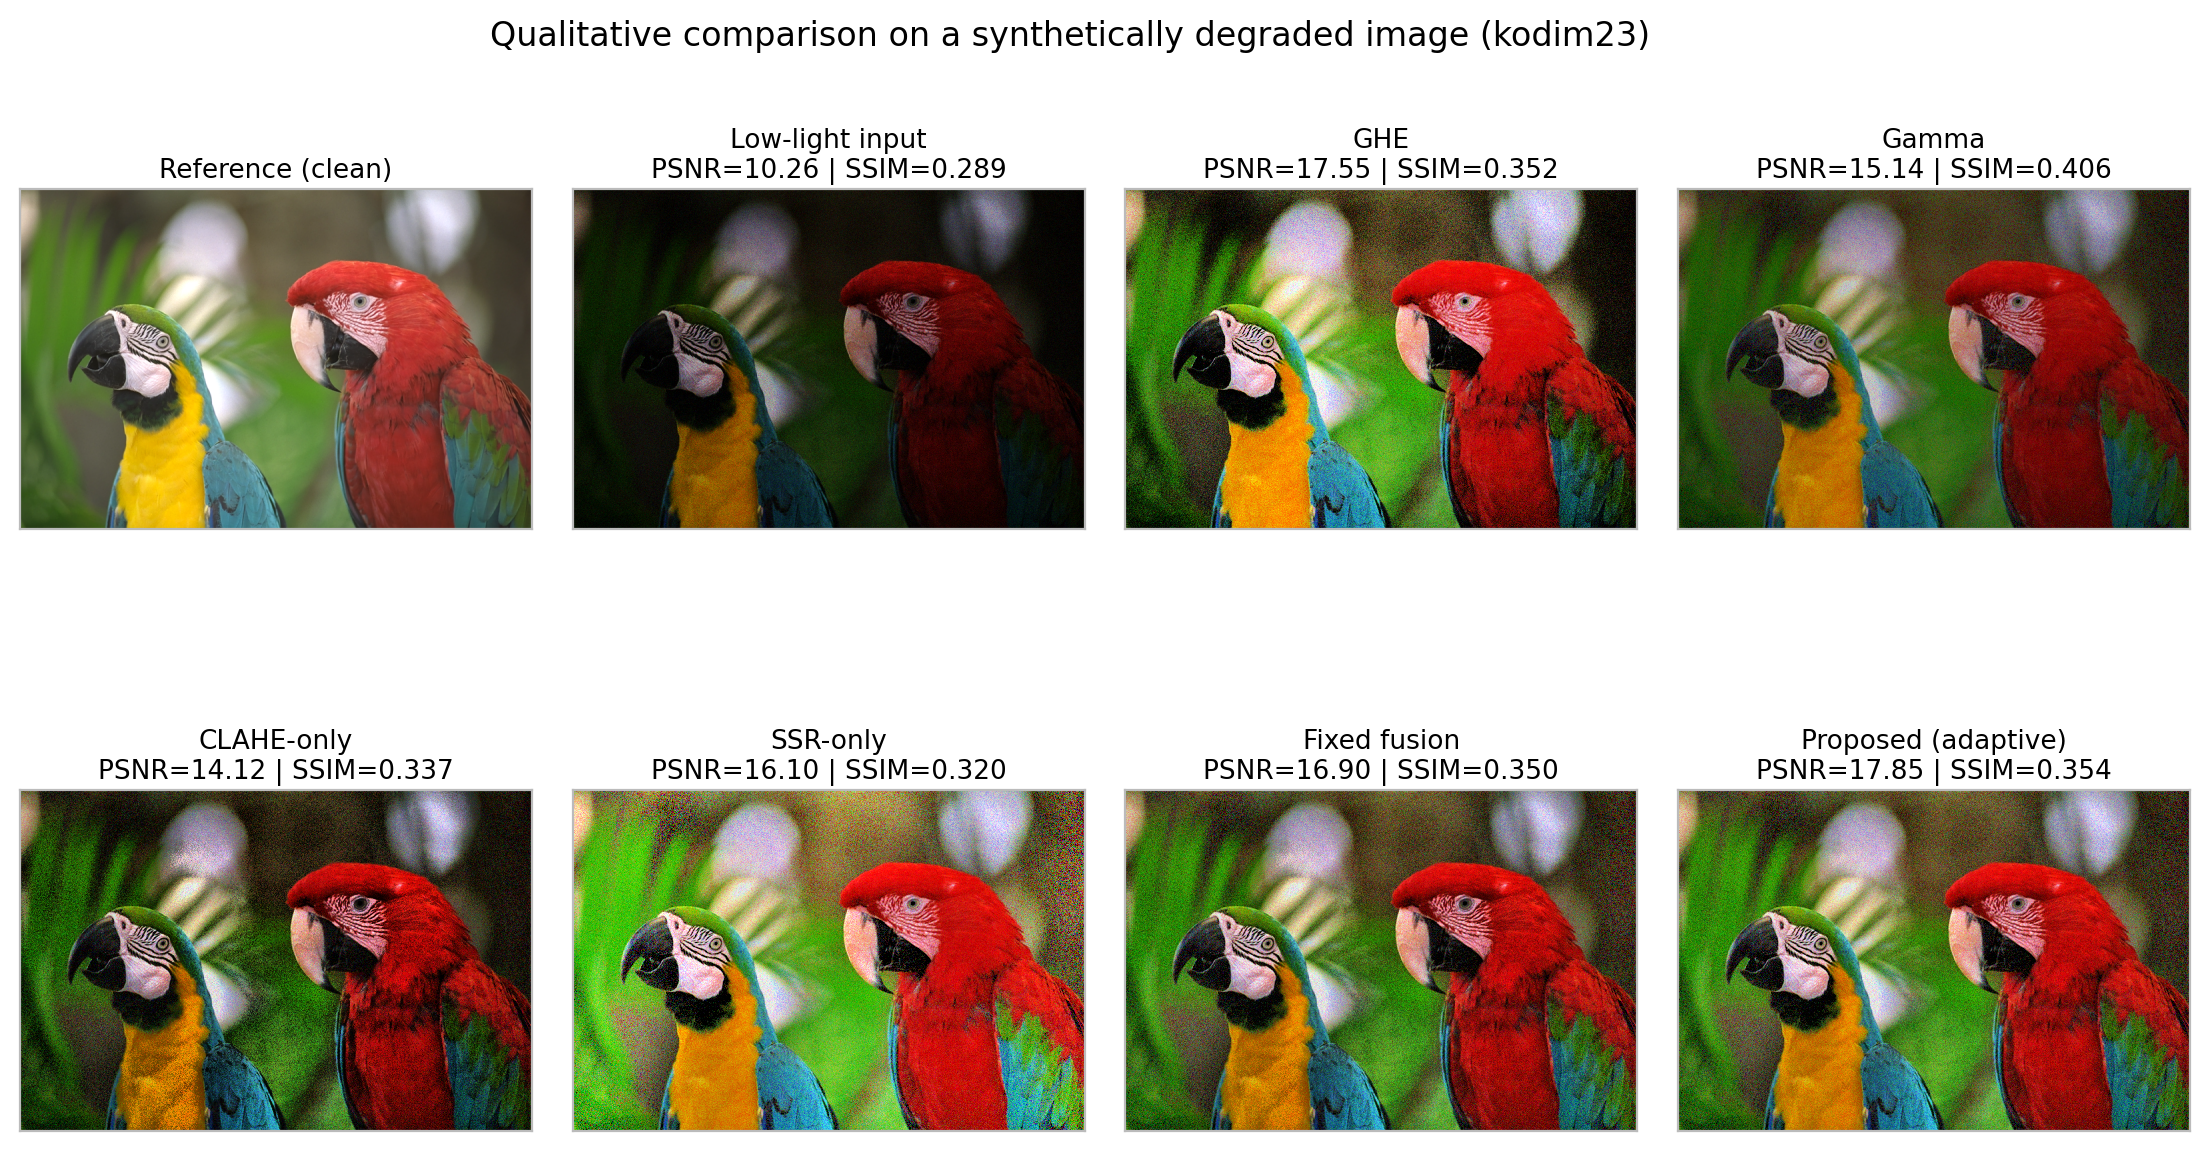
\includegraphics[width=\textwidth]{fig_qualitative.png}
\caption{Qualitative comparison on a synthetically degraded Kodak image
(kodim23). GHE and SSR-only visibly amplify background noise and SSR-only shifts
colors (green/magenta cast), while Gamma remains dark in shadows. Both fusions
restore brightness and contrast with natural color, and the adaptive method
edges out the fixed fusion in PSNR/SSIM. Values are for this specific sample
(seed~0).}
\label{fig:qual}
\end{figure*}

\begin{figure*}[t]
\centering
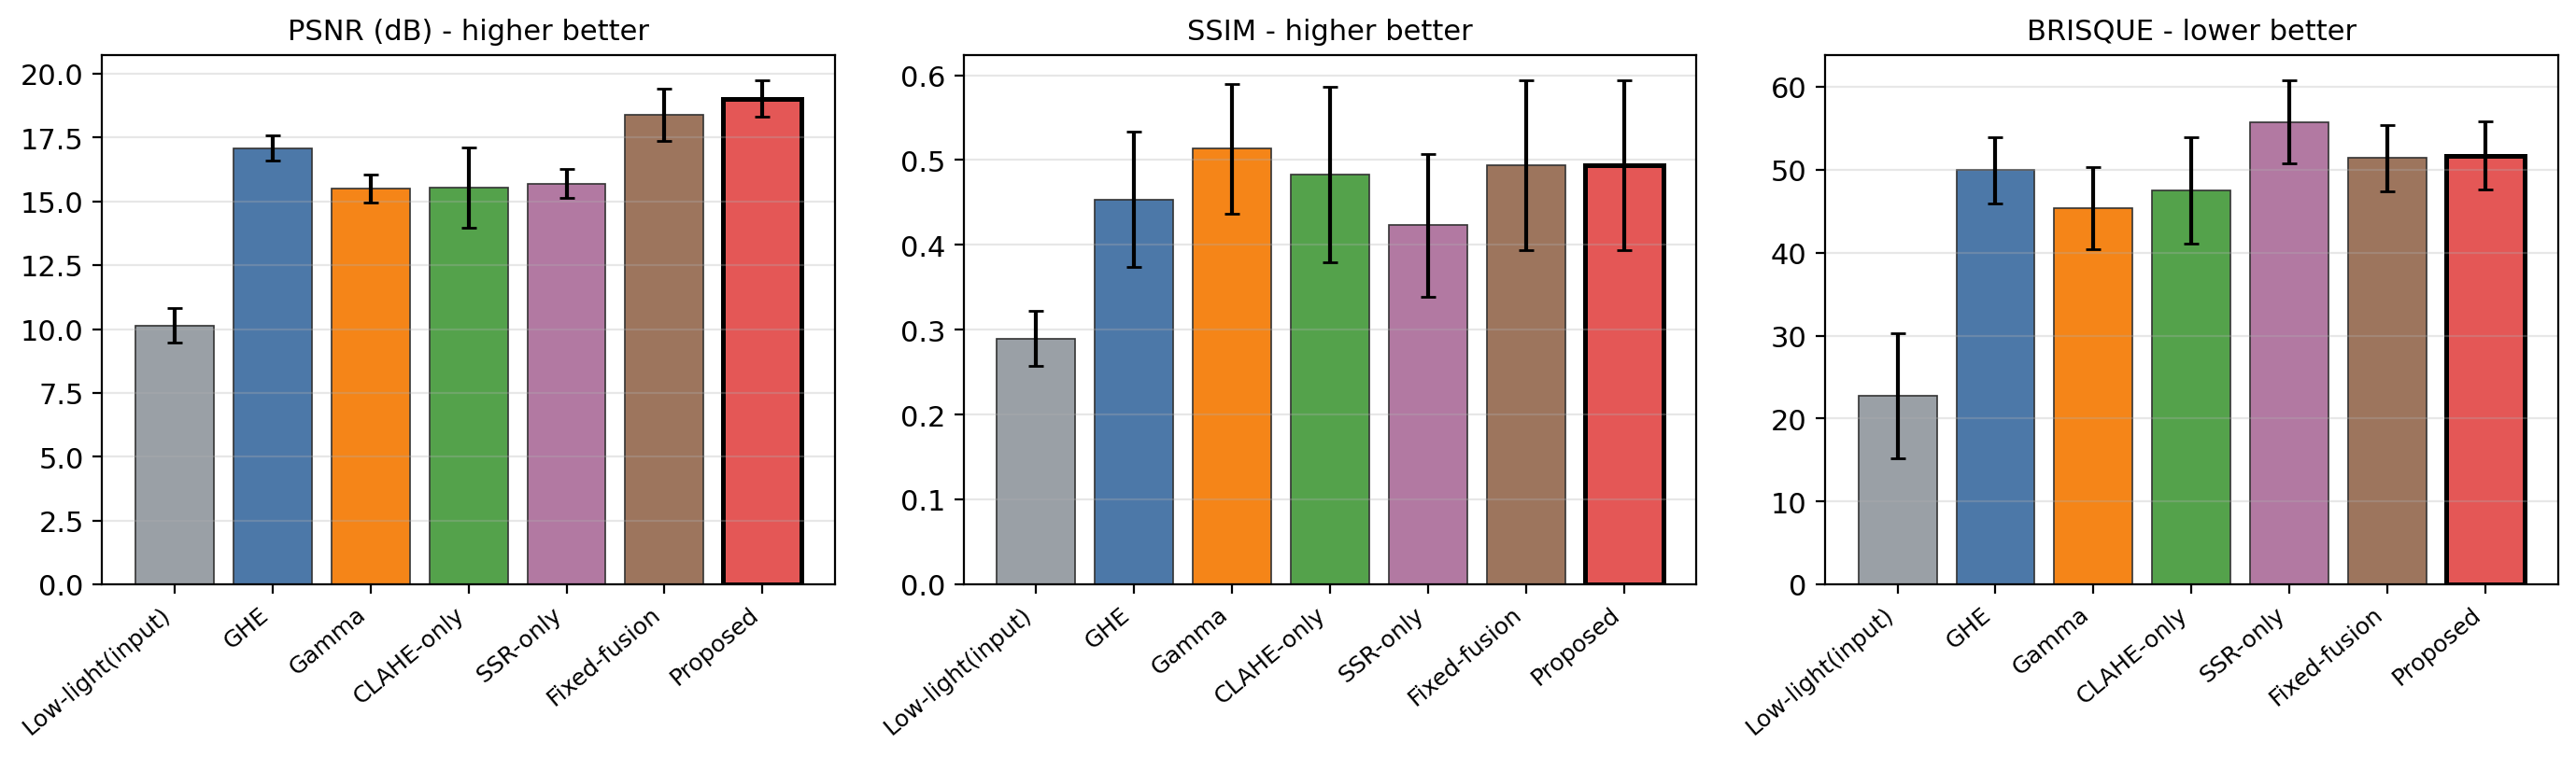
\includegraphics[width=\textwidth]{fig_metrics_bar.png}
\caption{Per-metric comparison with standard-deviation error bars across all
samples. The proposed adaptive method (outlined) leads on PSNR, just above the
fixed-weight fusion; Gamma leads on SSIM; the adaptive method's BRISQUE stays
below the SSR-only branch, reflecting suppression of Retinex artifacts.}
\label{fig:bars}
\end{figure*}

\subsection{Qualitative Comparison}
Fig.~\ref{fig:qual} shows a representative example. The low-light input is dark
with noticeable noise in shadow areas. GHE brightens aggressively but reveals
grain in flat regions. Gamma keeps colors natural but leaves shadow regions
under-exposed. CLAHE-only sharpens local contrast yet keeps some shadow noise,
and SSR-only recovers the most detail but exhibits a visible color cast and
amplified high-frequency noise. Both fusion variants combine the strengths:
brighter mid-tones and recovered detail from SSR, bounded contrast from CLAHE,
and preserved hue/saturation from the HSV design. The adaptive variant further
suppresses noise in the darkest regions (where it leans on CLAHE) while keeping
SSR detail in the lit foreground, yielding the highest fidelity.
Figs.~\ref{fig:qual2} and~\ref{fig:qual3} show two additional scenes. On
kodim05 (Fig.~\ref{fig:qual2}) the structured indoor content benefits clearly
from the recovered local contrast, and on kodim19 (Fig.~\ref{fig:qual3}), a
scene with a large bright sky region where a global stretch is naturally
competitive, the adaptive method still attains the best PSNR by avoiding
over-amplification in the darker foreground. Fig.~\ref{fig:bars} visualizes the
aggregate trends with error bars.

\begin{figure*}[t]
\centering
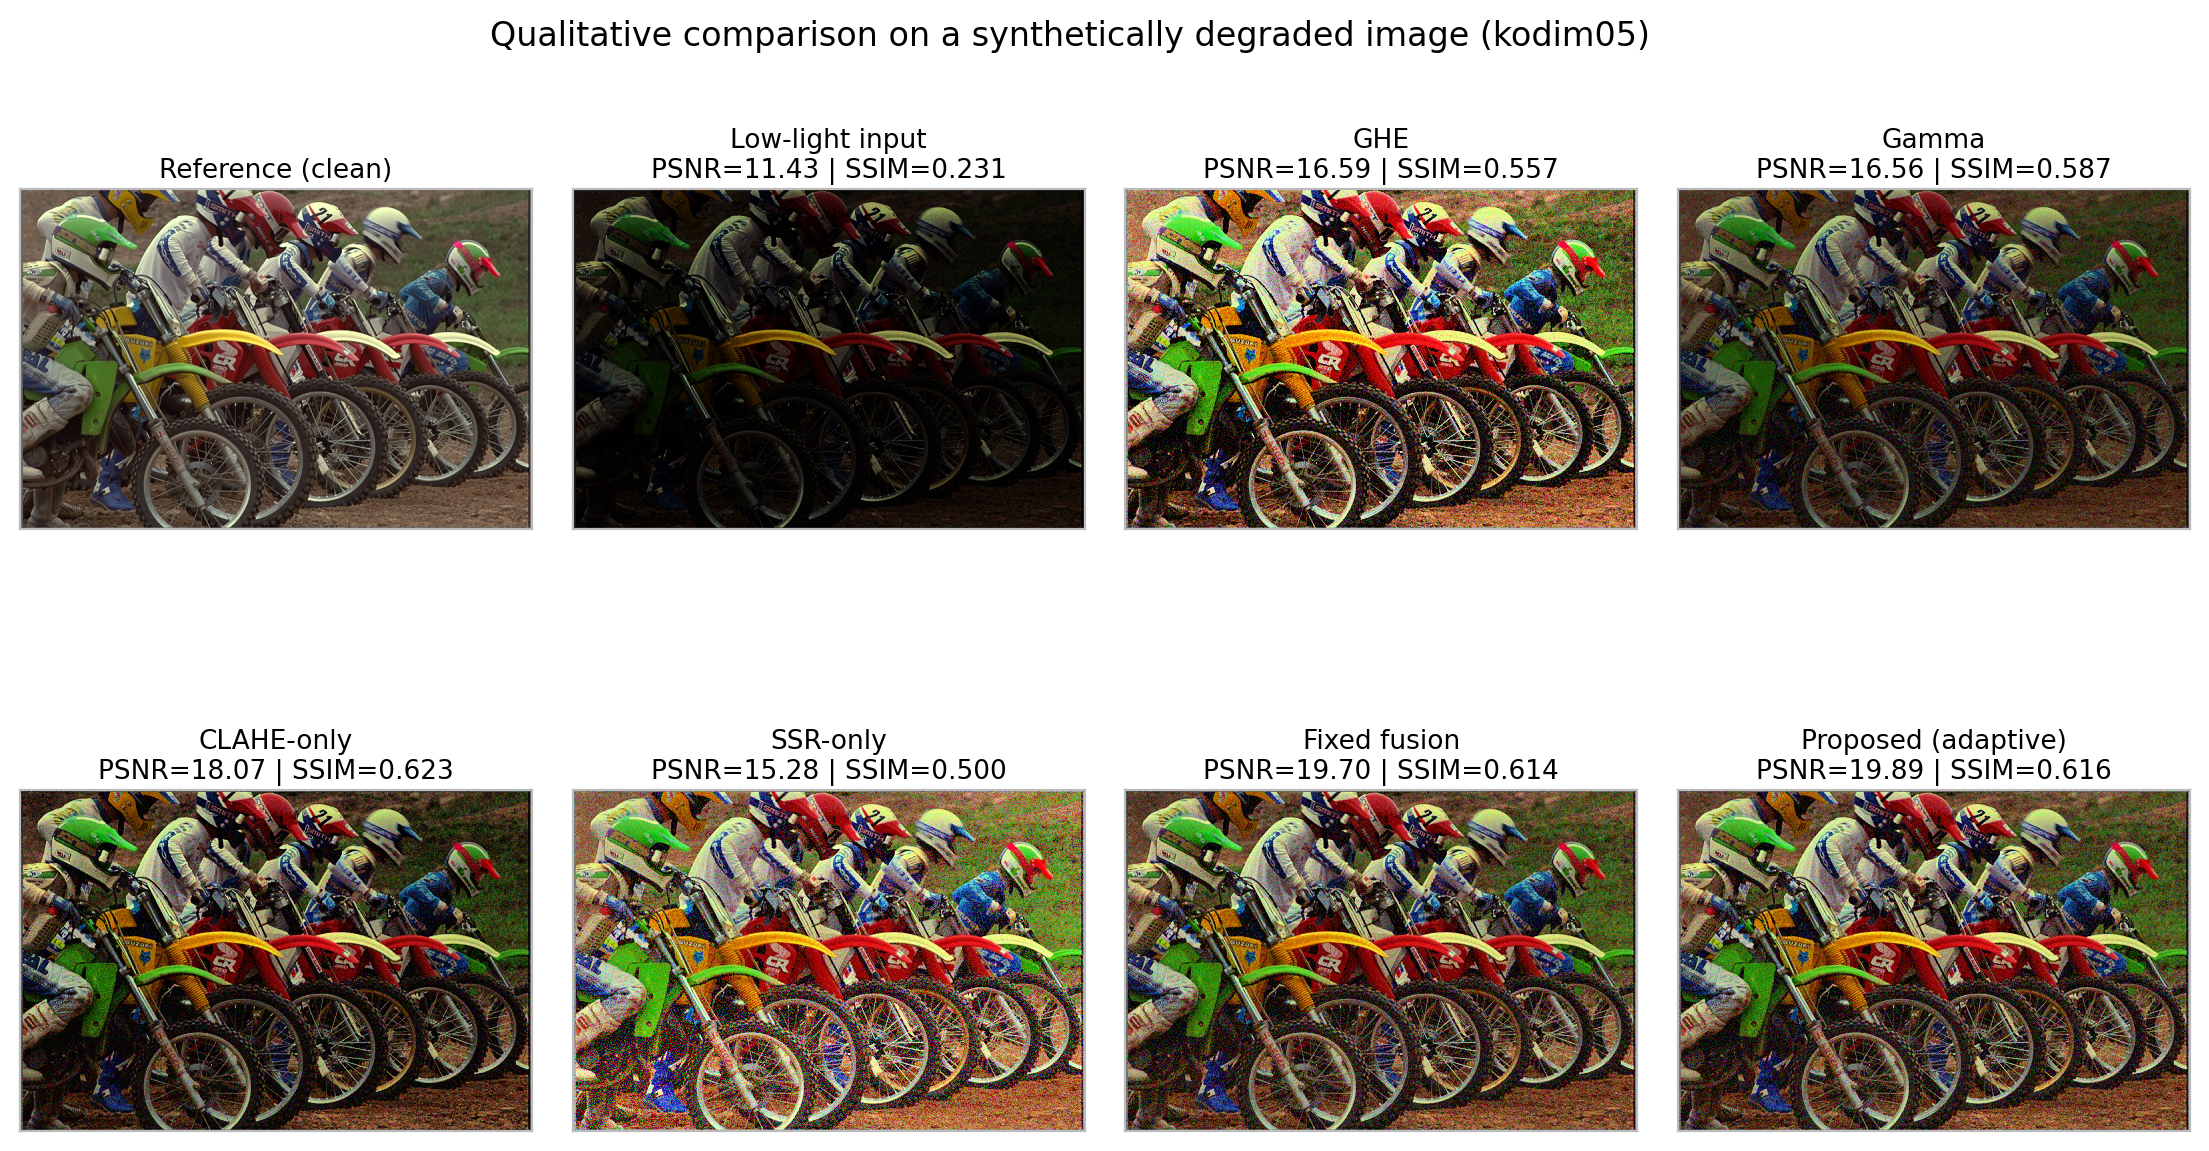
\includegraphics[width=\textwidth]{fig_qualitative2.png}
\caption{Additional qualitative comparison (kodim05). The adaptive method
recovers indoor structure and contrast while keeping color natural; SSR-only
again shows the strongest color cast and noise.}
\label{fig:qual2}
\end{figure*}

\begin{figure*}[t]
\centering
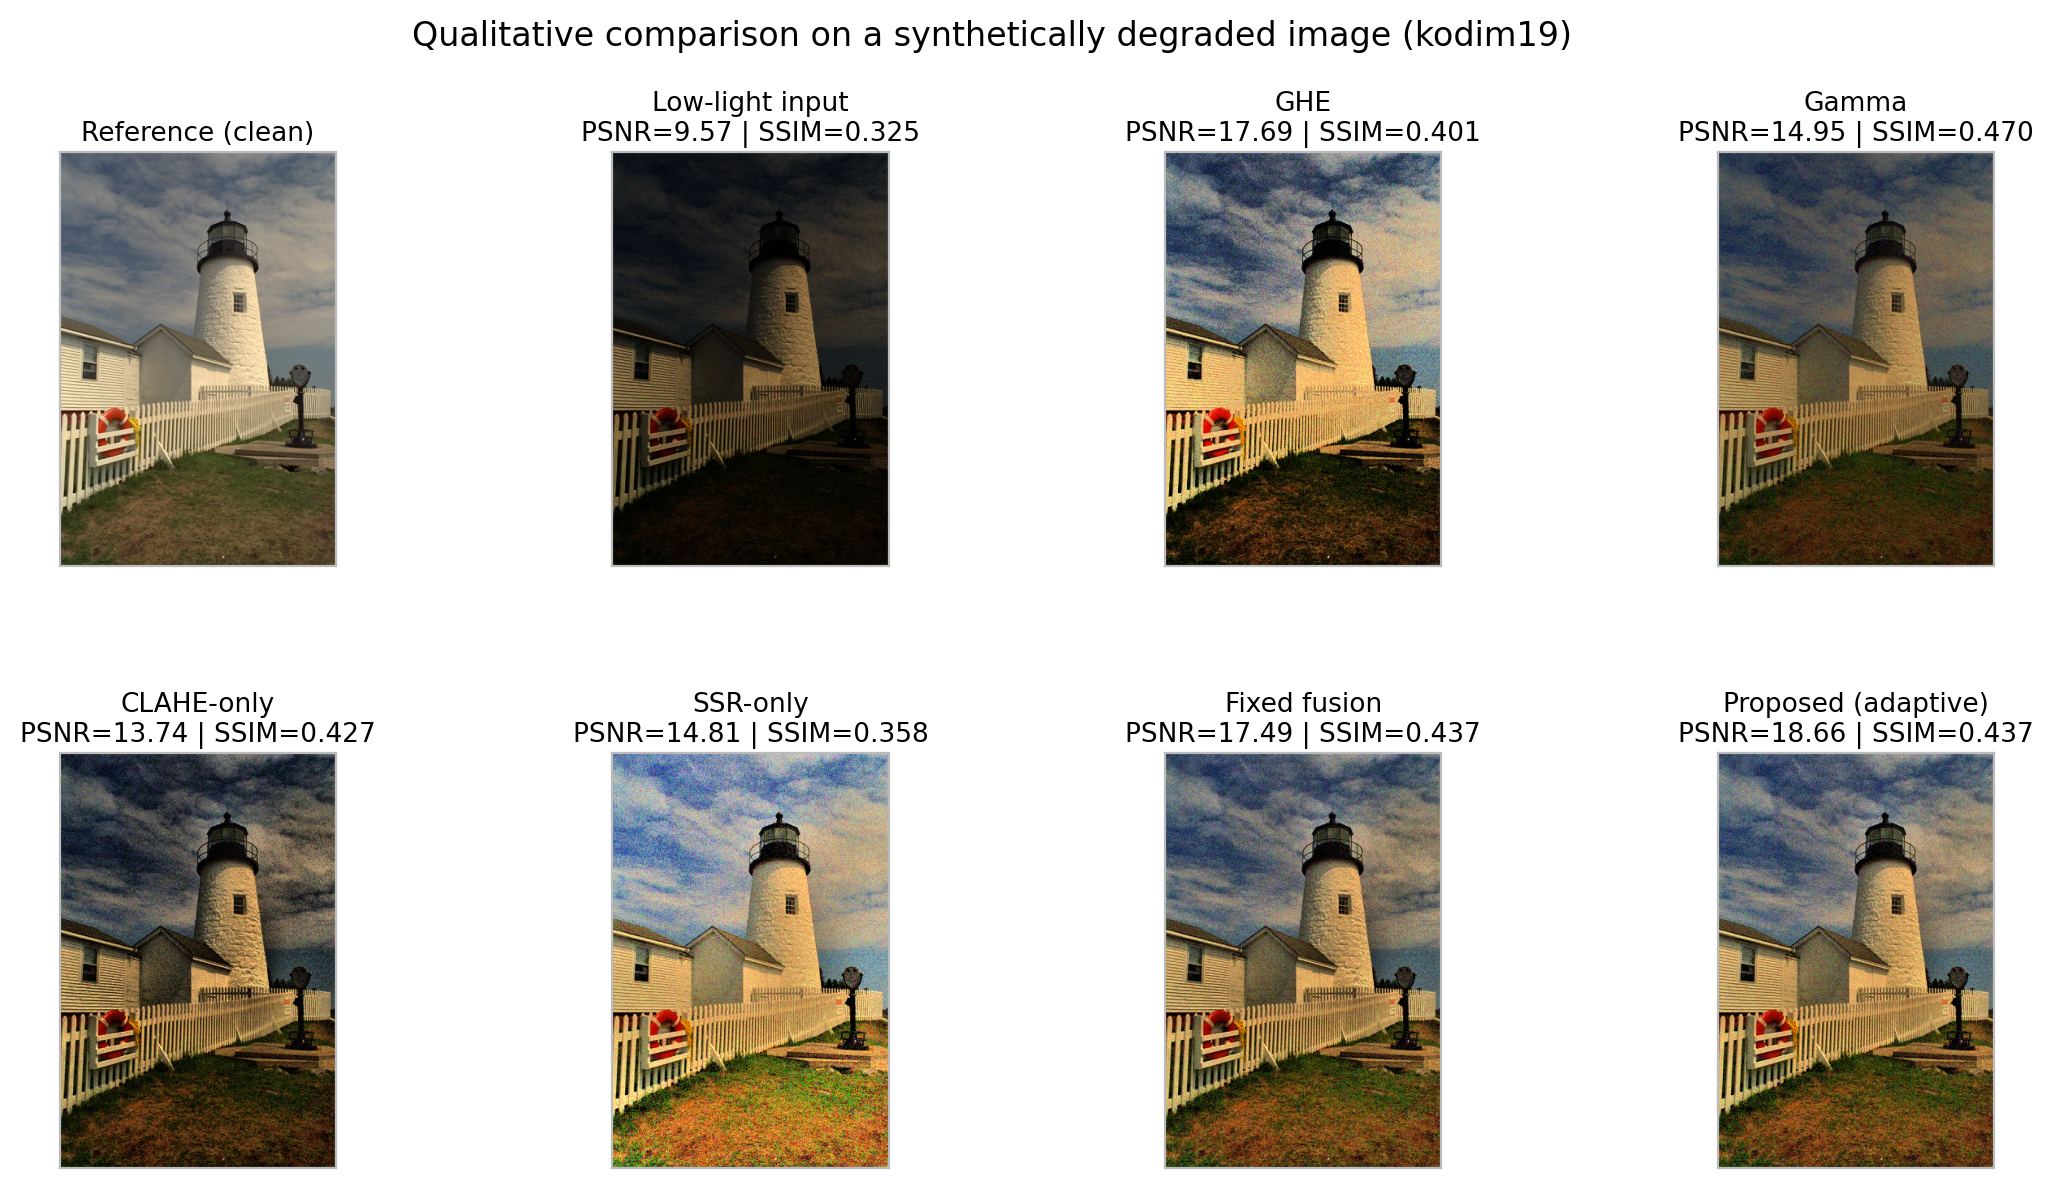
\includegraphics[width=\textwidth]{fig_qualitative3.png}
\caption{Additional qualitative comparison (kodim19), a bright-sky scene that
favors global stretching. The adaptive method still leads on PSNR by limiting
noise amplification in the darker foreground rather than stretching globally.}
\label{fig:qual3}
\end{figure*}

\subsection{Hyperparameter Study and Ablation}
Table~\ref{tab:hyper} and Fig.~\ref{fig:hyper} report the sensitivity of the
proposed adaptive method to its three factors, optimized using the fast
full-reference metrics.

\textbf{CLAHE clip limit $\beta$.} Increasing $\beta$ from $2$ to $4$ raises
PSNR ($18.89\rightarrow19.03$) as more contrast is recovered, but $\beta=8$
over-amplifies noise and reduces both PSNR ($17.76$) and SSIM ($0.459$). A
moderate $\beta=2$--$4$ is best; $\beta=2$ maximizes SSIM ($0.516$) and
$\beta=4$ maximizes PSNR.

\textbf{SSR Gaussian scale $\sigma$.} Larger surrounds give marginally higher
PSNR ($\sigma=80$ reaches $19.07$) because a wider surround estimates
illumination more smoothly and introduces fewer local halos; the effect is
mild, so a mid-range $\sigma=30$ is a safe default.

\textbf{Adaptive exponent $k$.} This is the key parameter of the proposed
fusion and exhibits a clean trade-off. Small $k$ lets SSR contribute even in
dim regions, which raises detail but also noise; large $k$ confines SSR to the
brightest regions, increasing SSIM ($k=0.8$ gives $0.504$) at a cost in PSNR
($17.31$). The best PSNR is at $k=0.35$ ($19.03$), which we adopt as the
default; $k\approx0.5$ offers a slightly higher SSIM ($0.503$) at a small PSNR
cost and is a reasonable alternative. That $k$ traces a monotonic
fidelity-vs-structure curve confirms that the illumination-driven weighting is
behaving as designed rather than acting arbitrarily.

The ablation is embedded in Table~\ref{tab:summary}: neither branch alone
matches either fusion. CLAHE-only and SSR-only reach only $15.55$ and
$15.70$\,dB PSNR, the fixed-weight fusion reaches $18.39$\,dB, and the
content-adaptive fusion reaches $19.03$\,dB. Two effects are visible: (i) fusing
the branches is strongly super-additive (CLAHE controls noise where SSR would
amplify it, and SSR restores detail where CLAHE alone is flat), and (ii) making
the fusion weight content-adaptive adds a further $0.64$\,dB over the best fixed
weight, isolating the value of the proposed weighting rule.

\subsection{Per-Image Consistency}
To verify that the average gain is not driven by a single favorable scene,
Table~\ref{tab:perimage} reports the mean PSNR per Kodak image (averaged over
the three noise realizations). The proposed adaptive method ranks first on
\emph{all five} images, including kodim19 -- a bright-sky scene where global
stretching is naturally competitive and where the fixed-weight fusion was beaten
by GHE. By leaning on CLAHE in the darker foreground instead of stretching
globally, the adaptive method recovers the lead there ($18.66$ vs.\ GHE's
$17.69$). This consistency indicates the benefit is robust across diverse
natural content (foliage, indoor structure, bright-sky scenes) rather than an
artifact of averaging.

\begin{table}[t]
\centering
\caption{Mean PSNR (dB) per Kodak image over 3 noise realizations.
Best per row in \textbf{bold}. Fix.\ = fixed-weight fusion; Prop.\ = proposed
adaptive fusion.}
\label{tab:perimage}
\setlength{\tabcolsep}{2.6pt}
\begin{tabular}{lccccccc}
\toprule
Image & Input & GHE & Gamma & CLAHE & SSR & Fix. & Prop. \\
\midrule
kodim01 & 9.71  & 16.48 & 15.43 & 16.32 & 16.06 & 18.86 & \textbf{19.16} \\
kodim05 & 11.43 & 16.59 & 16.56 & 18.08 & 15.28 & 19.70 & \textbf{19.90} \\
kodim07 & 9.76  & 17.12 & 15.41 & 15.49 & 16.26 & 18.99 & \textbf{19.57} \\
kodim19 & 9.57  & 17.69 & 14.95 & 13.74 & 14.80 & 17.49 & \textbf{18.66} \\
kodim23 & 10.26 & 17.56 & 15.14 & 14.12 & 16.09 & 16.91 & \textbf{17.86} \\
\midrule
Mean    & 10.14 & 17.09 & 15.50 & 15.55 & 15.70 & 18.39 & \textbf{19.03} \\
\bottomrule
\end{tabular}
\end{table}

\begin{table}[t]
\centering
\caption{Hyperparameter study for the proposed method (one factor varied at a
time around the default; mean over all samples).}
\label{tab:hyper}
\begin{tabular}{llcc}
\toprule
Factor & Value & PSNR$\uparrow$ & SSIM$\uparrow$ \\
\midrule
CLAHE clip limit $\beta$ & 2.0 & 18.89 & \textbf{0.516} \\
                         & 4.0 (def.) & \textbf{19.03} & 0.494 \\
                         & 8.0 & 17.76 & 0.459 \\
\midrule
SSR scale $\sigma$       & 15  & 18.96 & 0.491 \\
                         & 30 (def.) & 19.03 & 0.494 \\
                         & 80  & \textbf{19.07} & 0.499 \\
\midrule
Adaptive exponent $k$    & 0.2 & 18.67 & 0.474 \\
                         & 0.35 (def.) & \textbf{19.03} & 0.494 \\
                         & 0.5 & 18.53 & 0.503 \\
                         & 0.8 & 17.31 & \textbf{0.504} \\
\bottomrule
\end{tabular}
\end{table}

\begin{figure*}[t]
\centering
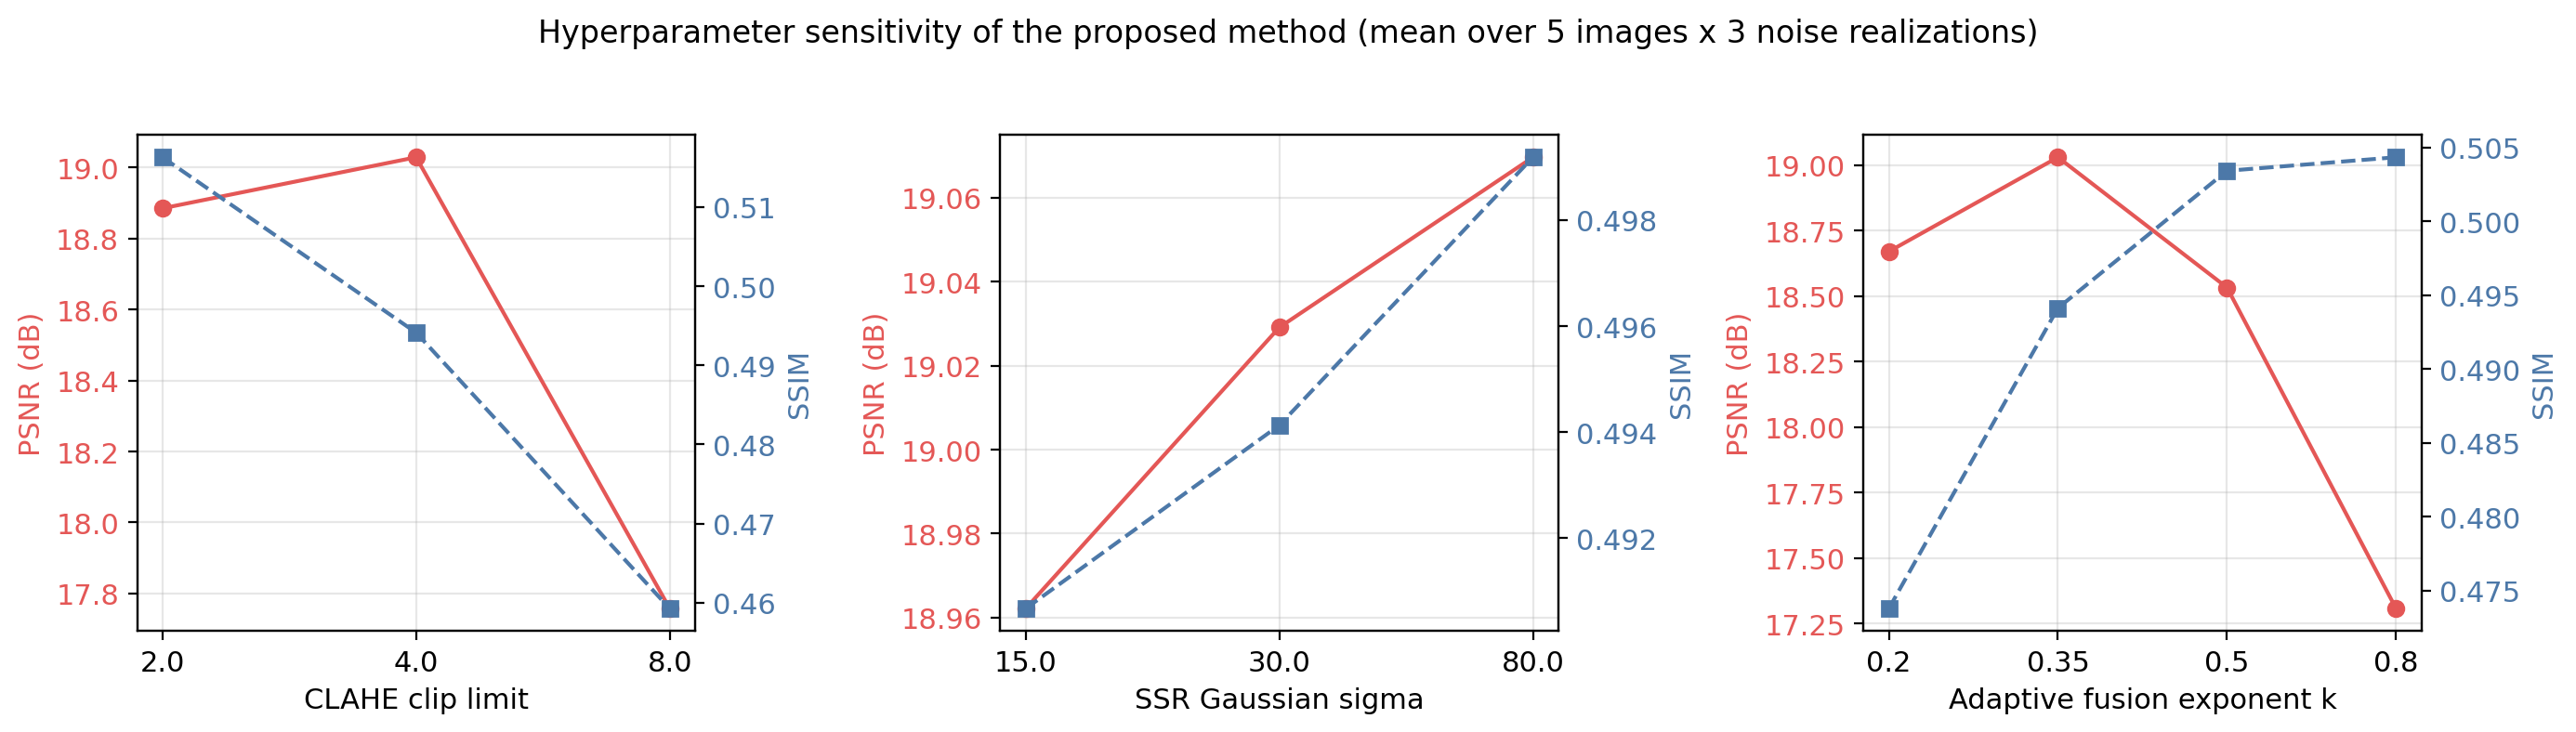
\includegraphics[width=\textwidth]{fig_hyperparams.png}
\caption{Hyperparameter sensitivity of the proposed adaptive method. Left:
CLAHE clip limit; middle: SSR Gaussian scale; right: adaptive fusion exponent
$k$. PSNR (red, left axis) and SSIM (blue, right axis) reveal the
contrast--fidelity trade-off; $k$ in particular traces a clean monotonic
trade-off between fidelity and structure.}
\label{fig:hyper}
\end{figure*}

\subsection{Discussion}
Three observations follow from the results. First, the relationship between PSNR
and BRISQUE is not monotonic: SSR-only attains a competitive PSNR ($15.70$\,dB)
yet the worst BRISQUE ($55.8$), because its halos and color shifts are
structured distortions that natural-scene-statistics penalize even when
pixel-wise error is moderate. Both fusions trade a little of SSR's raw detail
for a large reduction in these perceptual artifacts. Second, the SSIM advantage
of Gamma is a conservative-baseline effect: a smooth global curve cannot create
false structure, so it scores well on a structural metric while still leaving
the image visibly dark and noisy -- a reminder that no single metric is
sufficient and that PSNR, SSIM, and BRISQUE must be read together. Third, and
most relevant to the design, making the fusion weight content-adaptive yields a
consistent improvement over the best fixed weight (+$0.64$\,dB mean PSNR, and a
win on every individual image including the bright-sky scene that previously
favored a global stretch). This supports the central hypothesis: the
reliability of the CLAHE and SSR branches is spatially varying, and a per-pixel
illumination-driven weight exploits that structure where a single global weight
cannot. For nighttime surveillance the practical outcome is brighter, denoised,
color-faithful frames -- what downstream detectors and license-plate readers
need -- from a training-free, linear-time, CPU-only pipeline that can plausibly
run on edge hardware.

\section{Conclusion}
We presented a lightweight, training-free CLAHE--Retinex method for low-light
image enhancement that fuses a contrast-enhanced and a reflectance-recovered
Value channel in HSV space while preserving color. Its distinguishing feature is
a \emph{content-adaptive} fusion in which the per-pixel CLAHE/SSR weight is set
from a local illumination estimate through a single interpretable exponent,
rather than a fixed global blend. On a synthetic Kodak low-light benchmark the
adaptive method achieved the best PSNR among all compared methods
($19.03$\,dB), beating an otherwise-identical fixed-weight fusion by
$0.64$\,dB and the strongest classical baseline by $1.94$\,dB, and ranking first
on every individual image. The ablation showed both that fusing the branches is
super-additive and that the adaptivity itself contributes a further measurable
gain, while the hyperparameter study identified moderate clip limits,
mid-to-large SSR scales, and an exponent of $k\!\approx\!0.35$ as the most
effective regime.

\textbf{Limitations.} The evaluation uses synthetically degraded natural images
rather than real captured nighttime surveillance footage, so absolute scores
may not transfer directly; SSR uses a single fixed scale; the adaptive weight
depends only on a smoothed luminance estimate (not on a true noise or texture
estimate); and SSIM slightly favors the conservative Gamma baseline, indicating
the fusion can still introduce minor structural deviation.

\textbf{Future work.} Promising directions include multi-scale Retinex (MSR)
with color restoration, deriving the fusion weight from a local
noise/texture estimate rather than luminance alone, validation on real low-light
datasets (e.g., LOL, ExDark) and on downstream detection accuracy, and a learned
but lightweight selection of $\beta$, $\sigma$, and the adaptive exponent $k$.

\section*{Acknowledgment}
Generative AI tools (ChatGPT and Gemini) were used to help structure the report
and improve the clarity of the academic writing. All experiments, code,
results, and analyses were produced and verified by the author, who takes full
responsibility for the accuracy and integrity of the final work. All cited
references were checked against their original sources and DOIs.

\begin{thebibliography}{00}
\bibitem{pizer1987ahe} S. M. Pizer \emph{et al.}, ``Adaptive histogram
equalization and its variations,'' \emph{Comput. Vis. Graph. Image Process.},
vol. 39, no. 3, pp. 355--368, 1987, doi: 10.1016/S0734-189X(87)80186-X.

\bibitem{zuiderveld1994clahe} K. Zuiderveld, ``Contrast limited adaptive
histogram equalization,'' in \emph{Graphics Gems IV}, P. S. Heckbert, Ed.
Academic Press, 1994, pp. 474--485, doi: 10.1016/B978-0-12-336156-1.50061-6.

\bibitem{jobson1997retinex} D. J. Jobson, Z. Rahman, and G. A. Woodell,
``Properties and performance of a center/surround retinex,'' \emph{IEEE Trans.
Image Process.}, vol. 6, no. 3, pp. 451--462, 1997, doi: 10.1109/83.557356.

\bibitem{wang2004ssim} Z. Wang, A. C. Bovik, H. R. Sheikh, and E. P.
Simoncelli, ``Image quality assessment: from error visibility to structural
similarity,'' \emph{IEEE Trans. Image Process.}, vol. 13, no. 4, pp. 600--612,
2004, doi: 10.1109/TIP.2003.819861.

\bibitem{mittal2012brisque} A. Mittal, A. K. Moorthy, and A. C. Bovik,
``No-reference image quality assessment in the spatial domain,'' \emph{IEEE
Trans. Image Process.}, vol. 21, no. 12, pp. 4695--4708, 2012, doi:
10.1109/TIP.2012.2214050.

\bibitem{mittal2013niqe} A. Mittal, R. Soundararajan, and A. C. Bovik,
``Making a completely blind image quality analyzer,'' \emph{IEEE Signal
Process. Lett.}, vol. 20, no. 3, pp. 209--212, 2013, doi:
10.1109/LSP.2012.2227726.

\bibitem{ponomarenko2015tid2013} N. Ponomarenko \emph{et al.}, ``Image database
TID2013: Peculiarities, results and perspectives,'' \emph{Signal Process. Image
Commun.}, vol. 30, pp. 57--77, 2015, doi: 10.1016/j.image.2014.10.009.

\bibitem{guo2020zerodce} C. Guo \emph{et al.}, ``Zero-reference deep curve
estimation for low-light image enhancement,'' in \emph{Proc. IEEE/CVF Conf.
Comput. Vis. Pattern Recognit. (CVPR)}, 2020, pp. 1780--1789, doi:
10.1109/CVPR42600.2020.00185.

\bibitem{erakbiyik2026repo} B. Erakb{\i}y{\i}k, ``Hybrid CLAHE-Retinex
enhancement for nighttime surveillance images (source code),'' GitHub
repository, 2026. [Online]. Available:
\url{https://github.com/bekirerkbyk/hybrid-clahe-retinex}
\end{thebibliography}

\end{document}
